\documentclass{standalone}
\usepackage{pgfplots}
\pgfplotsset{compat=1.16}
\begin{document}
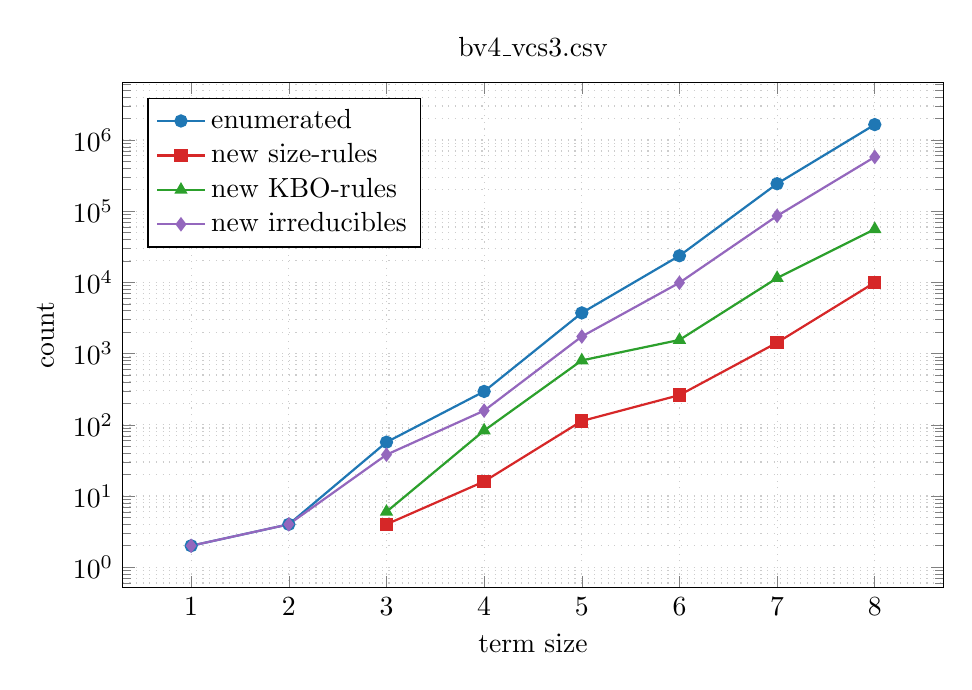
\begin{tikzpicture}
  \begin{axis}[
      width=12cm, height=8cm,
      xlabel={term size},
      ylabel={count},
      title={bv4\_vcs3.csv},
      ymode=log,
      grid=both,
      grid style={dotted, gray!40},
      legend pos=north west,
      legend cell align=left,
      mark size=2pt,
    ]
    \definecolor{cenumerated}{HTML}{1f77b4}
    \addplot[color=cenumerated, mark=*, thick] coordinates {(1,2) (2,4) (3,57) (4,294) (5,3728) (6,23644) (7,243051) (8,1643204)};
    \addlegendentry{enumerated}
    \definecolor{cnewsizerules}{HTML}{d62728}
    \addplot[color=cnewsizerules, mark=square*, thick] coordinates {(1,0) (2,0) (3,4) (4,16) (5,113) (6,261) (7,1425) (8,9960)};
    \addlegendentry{new size-rules}
    \definecolor{cnewkborules}{HTML}{2ca02c}
    \addplot[color=cnewkborules, mark=triangle*, thick] coordinates {(1,0) (2,0) (3,6) (4,83) (5,802) (6,1555) (7,11509) (8,55942)};
    \addlegendentry{new KBO-rules}
    \definecolor{cnewirreducibles}{HTML}{9467bd}
    \addplot[color=cnewirreducibles, mark=diamond*, thick] coordinates {(1,2) (2,4) (3,38) (4,158) (5,1738) (6,9885) (7,85901) (8,577187)};
    \addlegendentry{new irreducibles}
  \end{axis}
\end{tikzpicture}
\end{document}
